\documentclass{article}
\usepackage{fancyhdr}
\usepackage{extramarks}
\usepackage{amsmath}
\usepackage{amssymb}
\usepackage{enumerate}
\usepackage{graphicx}
\usepackage{pgfplotstable}
\usepackage{listings}
\lstset{framexleftmargin=5mm, frame=shadowbox, rulesepcolor=\color{blue}}


\topmargin=-0.45in
\evensidemargin=0in
\oddsidemargin=0in
\textwidth=6.5in
\textheight=9.0in
\headsep=0.25in

\linespread{1.1}

\pagestyle{fancy}
\lhead{\hmwkAuthorName}
\chead{\hmwkClass\ : \hmwkTitle}
\rhead{\firstxmark}
\lfoot{\lastxmark}
\cfoot{\thepage}

\renewcommand\headrulewidth{0.4pt}
\renewcommand\footrulewidth{0.4pt}

\setlength\parindent{24pt}

%
% Create Problem Sections
%

\newcommand{\enterProblemHeader}[1]{
    \nobreak\extramarks{}{Problem \arabic{#1} continued on next page\ldots}\nobreak{}
    \nobreak\extramarks{Problem \arabic{#1} (continued)}{Problem \arabic{#1} continued on next page\ldots}\nobreak{}
}

\newcommand{\exitProblemHeader}[1]{
    \nobreak\extramarks{Problem \arabic{#1} (continued)}{Problem \arabic{#1} continued on next page\ldots}\nobreak{}
    \stepcounter{#1}
    \nobreak\extramarks{Problem \arabic{#1}}{}\nobreak{}
}

\setcounter{secnumdepth}{0}
\newcounter{partCounter}
\newcounter{homeworkProblemCounter}
\setcounter{homeworkProblemCounter}{1}
\nobreak\extramarks{Problem \arabic{homeworkProblemCounter}}{}\nobreak{}

%
% Homework Problem Environment
%
% This environment takes an optional argument. When given, it will adjust the
% problem counter. This is useful for when the problems given for your
% assignment aren't sequential. See the last 3 problems of this template for an
% example.
%
\newenvironment{homeworkProblem}[1][-1]{
    \ifnum#1>0
        \setcounter{homeworkProblemCounter}{#1}
    \fi
    \section{Problem \arabic{homeworkProblemCounter}}
    \setcounter{partCounter}{1}
    \enterProblemHeader{homeworkProblemCounter}
}{
    \exitProblemHeader{homeworkProblemCounter}
}

%
% Homework Details
%   - Title
%   - Due date
%   - Class
%   - Section/Time
%   - Instructor
%   - Author
%

\newcommand{\hmwkTitle}{Homework\ \#10}
\newcommand{\hmwkDueDate}{April 27, 2015}
\newcommand{\hmwkClass}{PHYS 5243 - Solid State Physics}
\newcommand{\hmwkClassInstructor}{Professor Sheena Murphy}
\newcommand{\hmwkAuthorName}{Chase Brown}


\begin{document}

\begin{homeworkProblem}
	\section{Tight Binding Calculations for Single and Multi Layered Graphene: Comparison with ARPES data}

		\subsection{Single Layer Tight Binding Calculations}
			To begin, we start with the Brillouin Zone of Graphene, shown below.

			\begin{center}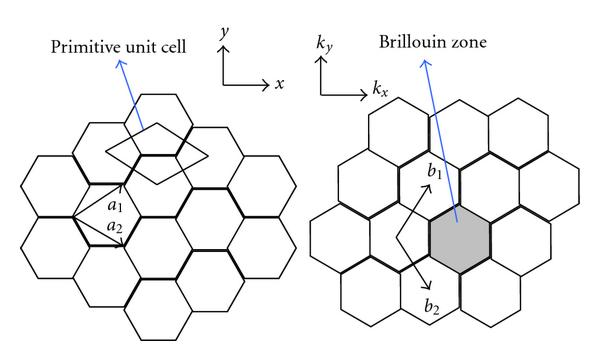
\includegraphics[scale=2]{BZ_Graphene.jpg}\end{center}
			
			The distance between carbon atoms in real space is $a = 0.142$ nm, therefore we can see that the primitive lattice vectors are $\textbf{a}_1 = \frac{a}{2} (3,\sqrt{3})$ and $\textbf{a}_2 = \frac{a}{2} (3,-\sqrt{3})$.  Taking the Fourier Transform of real space, we find that the lattice vectors for the reicprocal space are $\textbf{b}_1 = \frac{2\pi}{3a} (1,\sqrt{3})$ and $\textbf{b}_2 = \frac{2\pi}{3a} (1,-\sqrt{3})$. 
			
\end{homeworkProblem}
\end{document}
